
%\documentclass[13pt,revtex]{article}
%\documentclass[aps]{revtex4-1}
%\documentclass[11pt,A4]{revtex4-1}
\documentclass[10pt]{article}
\setlength{\columnsep}{0.75cm}
\usepackage{geometry}
 \geometry{
 letterpaper,
 total={210mm,297mm},
 left=30mm,
 right=30mm,
 top=30mm,
 bottom=30mm,
 }
\usepackage{amsmath,amsfonts,amssymb}
\usepackage{amsthm}
\usepackage{graphicx}
\usepackage{hyperref}
\usepackage{algorithm}
\usepackage{algorithmic}
\usepackage{bm} 

%\usepackage{pstricks}

\usepackage{amsmath}
\DeclareMathOperator\atanh{arctanh}


\def\be{\begin{equation}}
\def\ee{\end{equation}}


\linespread{1.0}

\newcommand{\arctanh}[1]{\mathrm{arctanh}#1}
\newcommand{\Sign}[1]{\mathrm{Sign}#1}

\def\<{\langle}
\def\>{\rangle}
\def\vx{\vec x}
\def\vh{\vec h}

\newcommand{\ud}{\mathrm{d}}
\newcommand{\etal}{\textit{ et. al. }}
\newcommand{\Ham}{\mathcal{H}}
\newcommand{\B}{\beta}
\def\matF{{\mathbb F}}
\def\Jij{J_{ij}}

\def\Imat{\mathbb{I}}
\def\ext{\qopname\relax m{ext}}

\newcommand{\mi}{\mathrm{i}}
\DeclareMathOperator{\Tr}{Tr}

%%%% 

\newcommand{\ddroit}{\textrm{d}}
% \newcommand{\eexp}{\text{e}}
\newcommand{\ie}{\emph{i.e.}$\;$}
\newcommand{\eg}{\emph{e.g.}$\;$}
\newcommand{\Ptot}{P(A_1\ldots A_L)}
\newcommand{\xz}{\vec{x}_0}
\newcommand{\xo}{\vec{x}_1}
\newcommand{\xt}{\vec{x}_2}
\newcommand{\Lam}{\bm{\Lambda}}
\newcommand{\Sig}{\bm{\Sigma}}
\newcommand{\HRule}{\rule{\linewidth}{0.5mm}}
\newcommand{\Xk}[1]{X^{\{#1\}}}
\newcommand{\xk}[1]{\vec{x}_{#1}}


\begin{document}
\title{Gaussian Phylogenetic reconstruction of correlations}
  
\author{Alejandro Lage-Castellanos, Pierre Barrat-Charlaix}
%\affiliation{Department of Theoretical Physics, Physics Faculty,
 % University of Havana, La Habana, CP 10400, Cuba. }
%\affiliation{``Henri Poincar\'e'' group of Complex Systems, University of Havana, Cuba. }
%\affiliation{CNRS, Laboratoire de Physique Statistique, {\'E}cole Normale Supérieure, 75005, Paris.}


\date{\today}

%\begin{abstract}

%\end{abstract}

\maketitle

\section{Direct problem: phylogenetic tree under gaussian evolution }

We consider a genome characterized by a vector $\vec x$ with an equilibrium probability distribution given by
\be
P(\vec x) =\frac 1 Z \exp H(\vec x) \qquad \mbox{with } \Ham(\vx) = \vx^T J \vx + \vh \cdot \vx \label{eq:equil}
\ee
where the degrees of freedom $x_i \in \mathbb R, i\in [1\ldots N]$ are continuous variables, and the interactions among them $\Jij$ are fixed, but randomly selected 
from a given ensemble of symmetric negative definite matrices. Notice the absense of the usual minus sign in front of the Hamiltonian. So, usually the vector $\vx$ will be near the maximum of $\Ham(\vx)$

We will assume that the matrix $J$ have some eigenvalues close to zero, so the genetic sequences can drift with relatively low cost in the subsapce generated by such eigenvectors. 

%Eventually, to achieve hiegher similarities with the phylogenetic reconstruction of protein families, we can assume that a part of the eigenvectors is done of couples of eigenvectors like this 
%\begin{eqnarray*}
%\vec e_{soft} &= (0,0,0,0,\alpha_i,0\ldots, 0,0,\alpha_k,0\ldots)  \qquad \mbox{ with low eigenvalue } \alpha \lesssim 0 \\
%\vec e_{hard} &= (0,0,0,0,\alpha_i,0\ldots, 0,0,-\alpha_k,0\ldots)  \qquad \mbox{ with big eigenvalue } \alpha \ll 0
%\end{eqnarray*}
%mimicking the fact that co-mutations of residues at positions $i$ and $k$, leaves unaltered the fitness of the proteins if they comutate in the correct directions, while they incurr in a big cost if they comutate in the wrong relative directions. But this later.

\subsection{Evolution process}

We consider a phylogenetic tree construction starting from a vector $\vx_0$ extracted randomly from the equilibrium distribution (\ref{eq:equil}). Then at every point of our evolution algorithm we do the following

\begin{algorithm} 
\caption{Generates tree of evolved vectors $T = \{\vx_0, \vx_{1,1}, \vx_{1,2}, \ldots\}$}
\begin{algorithmic}
\REQUIRE Root $\vx_0$, number of generations $G$, distance to mutants $d$.
\ENSURE Returns $T$
\STATE $T = \{ \vx_0 \}$  
\STATE $L = \{\vx_0 \} $  \COMMENT{Leaves of the tree (the last added nodes)}
\FOR{$(g=1; g<G; g+=1;)$}
  \STATE $L_{new} = \{\}$ 
  \FOR{($\vx$ in $L$)}
    \STATE $\vx_{\mbox{child1}} = \mbox{Monte-Carlo-evolve}(\vx, d)$
    \STATE $\vx_{\mbox{child2}} = \mbox{Monte-Carlo-evolve}(\vx, d)$
    \STATE Append $T \leftarrow= \{\vx_{\mbox{child1}}, \vx_{\mbox{child2}}\}$
    \STATE Append $L_{new} \leftarrow= \{\vx_{\mbox{child1}}, \vx_{\mbox{child2}}\}$
  \ENDFOR
  \STATE $L = L_{new}$
\ENDFOR
\RETURN $T = \{\vx_0, \vx_{1,1}, \vx_{1,2}, \ldots\}$
\end{algorithmic} \label{alg:1}
\end{algorithm}

The step named Monte-Carlo-evolve$(\vx,d)$, carries out a Monte Carlo evolution starting at configuration $\vx$  and until the configuration found  $\vx^t$ is at distance 
\[d = \frac 1 N ||\vx - \vx^t||_2 \]
This means that all new generation sequences are at the same distance of their parents.


\begin{figure*}[!htb]
\begin{center}
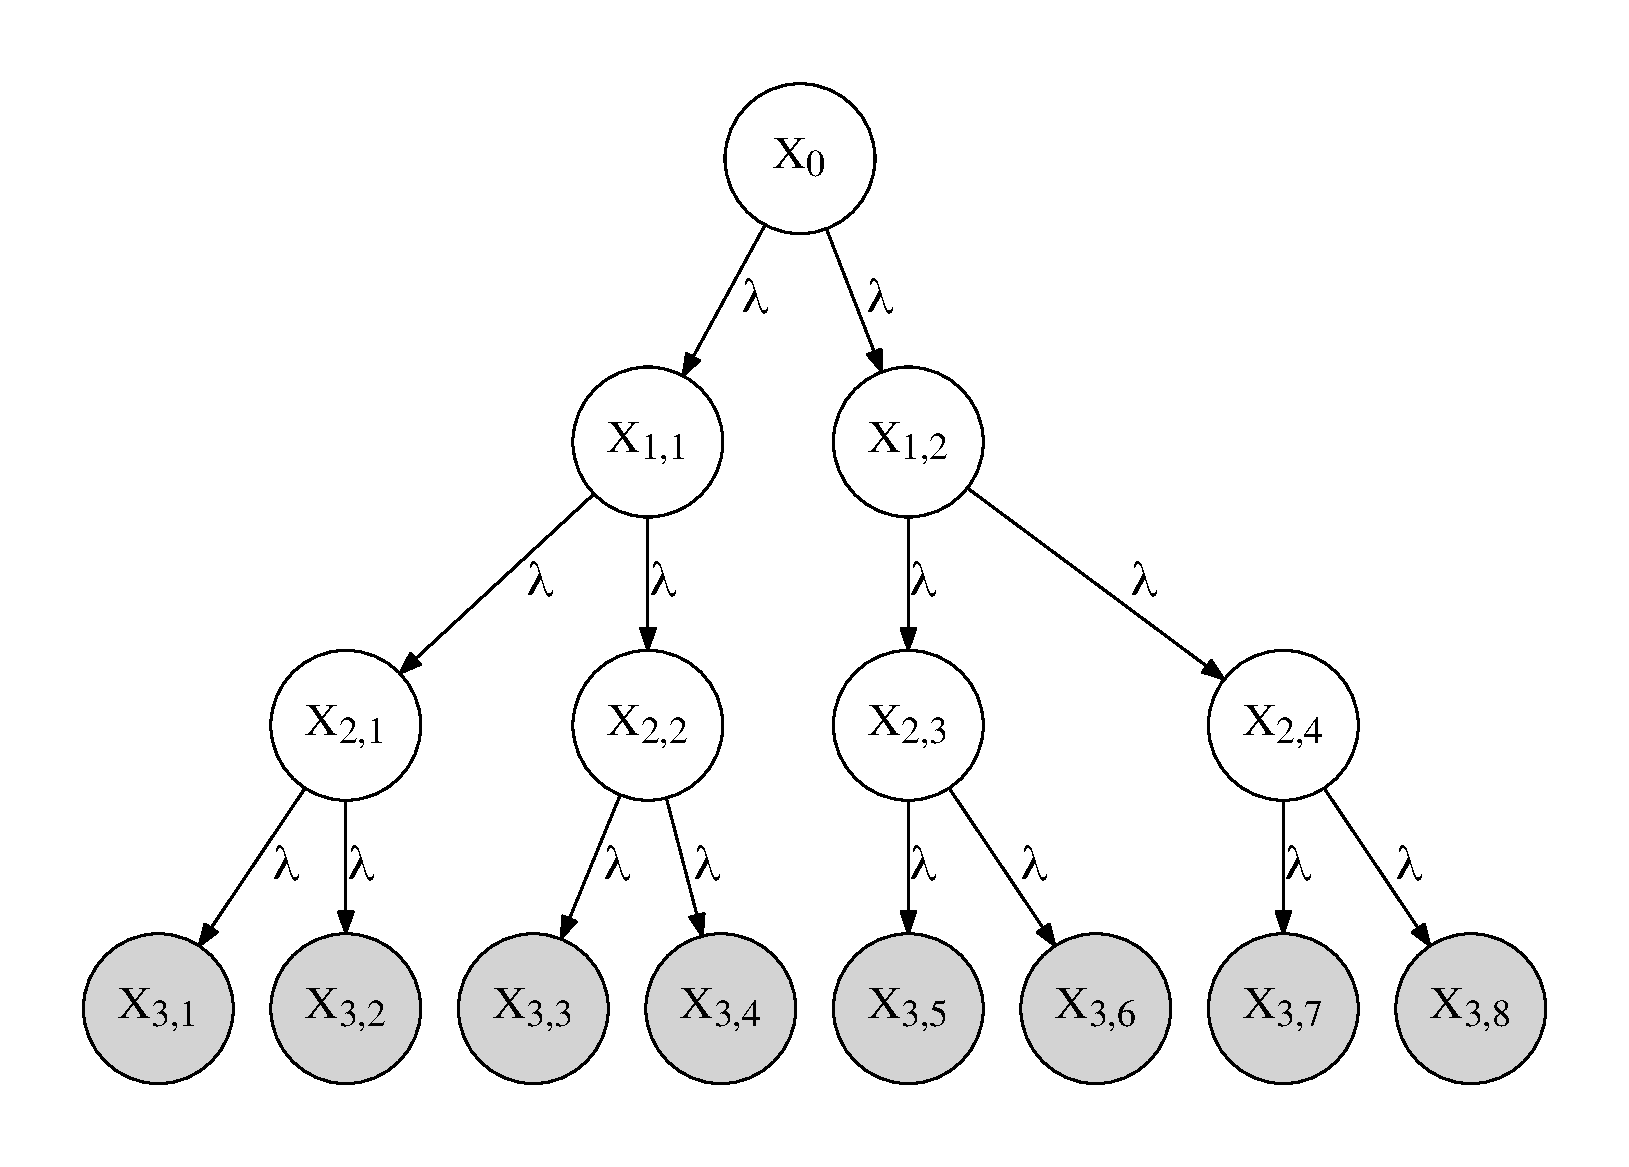
\includegraphics[width=0.65\textwidth]{Images/tree.pdf}
%  \includegraphics[width=\textwidth]{Images/regions.ps}
\end{center}
\caption{ Phylogenetic model for genetic drifting \label{fig:tree}}
\end{figure*}

\subsection{Likelihood of observed sequences}

In figure \ref{fig:tree} we represent the phylogenetic tree generated by an evolution process as described in algorithm \ref{alg:1}. The observed sequences are those of the last generation $\vx_{G,\cdot}$ and are portrayed in gray. We assume as known also the model $J,\vh$ and the distances $d$ at which the tree was created, but we ignore the set of sequences $\vx_{g,\cdot}$ in previous generations $g<G$.

Let us define the part of the interactions concerning a node and its children as follows
\be
K(\vx_0,\vx_{1,1},\vx_{1,2}) = \exp\left( \Ham(\vx_0) + \lambda_0 \vx_0 \cdot \vx_{1,1} + \lambda_0 \vx_0 \cdot \vx_{1,1} \right)
\ee
where the coupling constants $\lambda$ are there to ensure that the distance between the father and each children is consistently fixed to have the given expected value. 

The full probability distribution of the process in figure \ref{fig:tree} is 
\begin{eqnarray}
 P(T) &=& \frac 1 Z K(\vx_0,\vx_{1,1},\vx_{1,2}) K(\vx_{1,1},\vx_{2,1},\vx_{2,2}) K(\vx_{1,2},\vx_{2,3},\vx_{2,4}) \nonumber \\
      &&  K(\vx_{2,1},\vx_{3,1},\vx_{3,2}) K(\vx_{2,2},\vx_{3,3},\vx_{3,4})  \label{eq:PT} \\
      &&  K(\vx_{2,3},\vx_{3,5},\vx_{3,6}) K(\vx_{2,4},\vx_{3,7},\vx_{3,8}) \nonumber 
\end{eqnarray}
If this is correct, the marginal over any of these variables have to be the same distribution (\ref{eq:equil}). BUT IS NOT


\subsection{Reconstruction of hidden sequences}


\section{Ornstein-Uhlenbeck dynamics} % (fold)
\label{sec:ornstein_uhlenbeck_dynamics}

The system studied is the following. A tree -- balanced and binary in the following -- is given, with $K+1$ levels  and a time $\Delta t$ being assigned to each of its branches. A root configuration $\vec{x}$ is chosen with gaussian probability 
$$ P_{eq}(\vec{x}) = \frac{1}{\sqrt{(2\pi)^N \vert \bm{C}\vert}}\exp\left\{ -\frac{1}{2}\vec{x}^T\bm{C}^{-1}\vec{x} \right\}. $$ 
It then evolves using dynamics described below. At each division event of the tree, two copies of the system are created and evolve independently along each branch. The final result of the process are the configurations of the $2^K$ leaves of the tree. \\
The inference problem is the following. With the knowledge of the leaves configurations and of the type of evolution dynamics, is it possible to reconstruct the potential $\bm{C}^{-1}$ acting on the system? The idea for this is to
\begin{itemize}
  \item Compute the probability of observing leaves configurations given the potential $\bm{C}^{-1}$, $P(leaves\vert\bm{C})$.
  \item Invert this relation using Bayes formula: $$P(\bm{C}\vert leaves) = \frac{P(leaves\vert\bm{C})P(\bm{C})}{Z}$$
 \end{itemize}

\subsection{Dynamics} % (fold)
\label{sub:dynamics}


The Langevin equation for a $N$-dimensional particle with position $\vec{x} = (x_i),\;\;i\in\{1\ldots N\}$ in a harmonic potential centered in $\vec{0}$ is 
\begin{equation}
  \gamma \frac{\ddroit x_i}{\ddroit t} = -\sum_{j}\lambda_{ij}x_j + \sqrt{2kT\gamma}\xi_i(t)
\end{equation}
with $\langle \xi_i(t)\xi_j(t') \rangle = \delta_{ij}\delta(t-t')$. The diffusion coefficient is $D = kT/\gamma$. The force on the particle is represented by the stiffness matrix $\lambda_{ij}$. It can be shown that the corresponding Fokker-Planck equation is 
\begin{equation}
\label{eq:multiFP}
  \gamma\partial_t P = \left(-\sum_{i,j}\frac{\partial}{\partial x_i}\lambda_{ij}x_j + kT\frac{\partial^2}{\partial x_i^2}\right)P
\end{equation} 
The stationnary state solution of this is 
\begin{equation}
  P_{eq}(\vec{x}) = \frac{1}{\sqrt{(2\pi)^N \vert \bm{C}\vert}}\exp\left\{ -\frac{1}{2kT}\vec{x}^T\bm{C}^{-1}\vec{x} \right\}
\end{equation}
with $\bm{C}=\lambda^{-1}$. In other words, the potential the particle evolves in is $V(x)=\frac{1}{2}\vec{x}^T\bm{C}^{-1}\vec{x} = \frac{1}{2}\sum_{i,j} \lambda_{ij}x_i x_j$. For our case, we can set $kT=1$ for the rest.\\

Following \cite{singh2017multiOU}, we can explicitely write the solution of \ref{eq:multiFP}. The result is an Ornstein-Uhlenbeck process defined in the following way
\begin{equation}
  \label{eq:multiOU}
  \begin{split}
    P(\vec{x}) =& \frac{1}{\sqrt{(2\pi)^N \vert \bm{C}\vert}}\exp\left\{ -\frac{1}{2}\vec{x}^T\bm{C}^{-1}\vec{x} \right\},\\
    P(\vec{x}_2 | \vec{x}_1, \Delta t) =& \frac{1}{\sqrt{(2\pi)^N(1-e^{-2\Delta t})\vert\bm{\Sigma}^{-1}\vert}}\exp\left\{ -\frac{1}{2}(\vec{x}_2 - \vec{\mu_1})^T\bm{\Sigma}^{-1}(\vec{x}_2 - \vec{\mu_1}) \right\}.
  \end{split}
\end{equation}
where 
$$ \mu_1 = \Lam\vec{x}_1, \qquad \bm{\Sigma} = \bm{C} - \Lam\bm{C}\Lam, \qquad \Lam = e^{-\bm{\gamma C}^{-1}\Delta t}.$$ Thus, the average and covariance of variable $\vec{x}_1$ are time dependent through matrix $\Lam$, which itself depends on the equilibrium properties of the process through $\bm{C}$, and on the temporal dynamics through the dynamical parameter $\gamma$. It is important to notice that $\Lam$, $\bm{C}$ and $\bm{\Sigma}$ all commute and are symetric. \\

\textbf{Note}: On dimensions. $\bm{C}\sim [T^2]$, $\Lam\sim[T^{-2}]$, $\gamma\sim[T^{-1}]$ and $kT\sim[L^2T^{-2}]$.\\

What is the probability of observing two configurations $\vec{x}_1$ and $\vec{x}_2$ of the system knowing that they are separated by time $\Delta t$? Using the identity $\bm{C}^{-1} = \Sig^{-1}(1-\Lam^2)$, we find
\begin{equation}
  \label{eq:JointProbTwoVar}
  \begin{split}
    \log P(\vec{x}_2, \vec{x}_1, \Delta t) &\propto -\frac{1}{2}\left[ \xt^T\Sig^{-1}\xt - 2\xt^T\Sig^{-1}\Lam\xo + 2\xo^T\Lam\Sig^{-1}\Lam\xo + \xo^T\bm{C}^{-1}\xo \right]\\
          &\propto -\frac{1}{2}\left[ \xt^T\Sig^{-1}\xt + \xo^T\Sig^{-1}\xo - 2\xo^T(\Lam\Sig^{-1})\xt \right],
  \end{split}
\end{equation}
which is a gaussian distribution with a block correlation matrix, having $\Sig^{-1}$ on the diagonal blocks and $-\Lam\Sig^{-1}$ on the off-diagonal part. Inverting this matrix -- like a $2\times2$ matrix, since everything commutes -- yields the following expression for the covariance of configurations $\xo$ and $\xt$ separated by $\Delta t$:
\begin{equation}
  \langle\xo\xt^T\rangle = \Lam\Sig^{-1}\cdot\Sig^2(1-\Lam^2)^{-1} = \Lam \bm{C}.
\end{equation}

% subsection dynamics (end)

\subsection{Small trees} % (fold)
\label{sub:small_trees}

As an exercise, let us compute probability of the smallest non trivial tree, $ie$ root $\xz$ with children $\xo$ and $\xt$ and branch length $\Delta t$. The probability of observing given configurations on this topology is 
\begin{equation}
  \begin{split}
    P(\xz,\xo,\xt ; \Delta t) &= P(\xo\vert\xz)P(\xt\vert\xz)P(\xz)\\
    &\propto\exp-\frac{1}{2}\left\{ \xo\Sig^{-1}\xo + \xt\Sig^{-1}\xt - 2(\xo + \xt)\Sig^{-1}\Lam\xz + \xz\Sig^{-1}(1+\Lam^2)\xz \right\},
  \end{split}
\end{equation}
where the identity $\bm{C}^{-1} = \Sig^{-1}(1-\Lam^2)$ has been used.
Integrating this over all values of $\xz$ using eq.~(\ref{eq:GaussianIntegration}), and remembering that $\Sig(2\Delta t) = \bm{C} - \Lam^2\bm{C}\Lam^2$, we recover equation \ref{eq:JointProbTwoVar} with $\Delta t \rightarrow 2\Delta t$, that is with $\Lam\rightarrow\Lam^2$.

\textbf{Note}: Gaussian integration
\begin{equation}
  \label{eq:GaussianIntegration}
  \int\exp-\frac{1}{2}\left\{\vec{x}^TA\vec{x} + B^T\vec{x}\right\}\ddroit^{n}x = \left( \frac{(2\pi)^n}{\vert A\vert} \right)^{1/2}\exp\left(\frac{1}{8}B^TA^{-1}B\right)
\end{equation}

Let us do the same thing for a tree with two levels. Nodes are labelled from $0$ to $6$, with $\xk{1}$ and $\xk{2}$ being the children of root $\xk{0}$, and so on. The full probability can be written
\begin{equation}
  P(\{\xk{i}\}_{i=0\ldots 6}) = P(\xk{3},\xk{4}\vert\xk{1})P(\xk{5},\xk{6}\vert\xk{2})P(\xk{1}\vert\xk{0})P(\xk{2}\vert\xk{0})P_{eq}(\xk{0})
\end{equation}
Integrating this over $\xk{0}$ gives equation \ref{eq:JointProbTwoVar} for variables $1$ and $2$, with $\Delta t\rightarrow2\Delta t$, while the part concering variables $3$ to $6$ remains untouched. Thus, we have to perform the following integration.
\begin{equation}
  \label{eq:IntegrationTree2}
  \begin{split}
    P(\{\xk{i}\}_{i=3\ldots 6}) = \int\ddroit\xk{1}\ddroit\xk{2}&P(\xk{3},\xk{4}\vert\xk{1})P(\xk{5},\xk{6}\vert\xk{ 2})\cdot P(\vec{x}_2, \vec{x}_1, 2\Delta t)\\
    \propto \int\ddroit\xk{1}\ddroit\xk{2} \exp\,-\frac{1}{2}&\left\{ (\xk{3/4}-\Lam\xk{1})\bm{C}^{-1}(1-\Lam^2)^{-1}(\xk{3/4}-\Lam\xk{1}) +  (\xk{5/6}-\Lam\xk{2})\bm{C}^{-1}(1-\Lam^2)^{-1}(\xk{5/6}-\Lam\xk{2})\right.\\
    &\left. +\xk{1/2}\bm{C}^{-1}(1-\Lam^4)^{-1}\xk{1/2} -2\xk{1}\bm{C}^{-1}\Lam^2(1-\Lam^4)^{-1}\xk{2}  \right\}
  \end{split}
\end{equation}
where the notation $\xk{1/2}$ means that the corresponding term must be repeated for variables $1$ and $2$. For example, $\xk{1/2}\bm{U}\xk{1/2} = \xk{1}\bm{U}\xk{1} + \xk{2}\bm{U}\xk{2}$. Here, we used the fact that when $\Delta t\rightarrow2\Delta t$, $\Lam\rightarrow\Lam^2$.
Since we have to integrate over $1$ and $2$, let us count linear and quadratic terms in those parameters to apply eq~(\ref{eq:GaussianIntegration}). For instance, $\xk{1}$:
\begin{itemize}
  \item Quadratic: $2\bm{C}^{-1}\Lam^2(1-\Lam^2)^{-1} + \bm{C}^{-1}(1-\Lam^4)^{-1}$
  \item Linear: $ -2\bm{C}^{-1}\Lam(1-\Lam^2)(\xk{3}+\xk{4}) - 2\bm{C}^{-1}\Lam^2(1-\Lam^4)^{-1}\xk{2} $
\end{itemize}
From this point, it is quite clear that the result will be gaussian. The output of the integration will give quadratic and cross terms in $\xk{3/4/5/6}$, with a correlation matrix depending on $\bm{C}$ and $\Lam$. The exact expression has to be computed, though.  \\

Let's try in another way. Since matrices $\bm{C}$ and $\Lam$ commute, we can express all the previous equations as scalars ones. Eq~(\ref{eq:IntegrationTree2}) can formally be expressed as 
\begin{equation}
\label{eq:Tree2Scalar}
    P(\{\xk{i}\}_{i=3\ldots 6}) \propto \int\ddroit x_1\ddroit x_2 \exp-\frac{1}{2}\left\{\kappa \left(x_1^2+x_2^2\right) +2\nu x_1x_2 + 2\alpha_1 x_1 + 2\alpha_2 x_2 + c  \right\}
\end{equation}  
where
\begin{align*}
  \bm{C}\cdot\kappa &= 2\Lam^2(1-\Lam^2)^{-1} + (1-\Lam^4)^{-1},\\
  \bm{C}\cdot\alpha &= -\Lam(1-\Lam^2)^{-1},\;\text{with}\;\; \alpha_1 = \alpha(x_3+x_4) \;\text{and}\;\; \alpha_2 = \alpha(x_5+x_6),\\
  \bm{C}\cdot\nu &= -\Lam^2(1-\Lam^4)^{-1},\\
  \bm{C}\cdot c &= (1-\Lam^2)^{-1}(x_3^2+x_4^2+x_5^2+x_6^2).
\end{align*}
The integral can be computed easily, seeing that it is the integration of a vectorial gaussian variable $(x_1,x_2)$ with correlation matrix having $\kappa$ on the diagonal blocks and $\nu$ on the off-diagonal. Using (\ref{eq:GaussianIntegration}), we get
\begin{multline}
  \label{eq:Tree2HalfInt}
  P(\{\xk{i}\}_{i=3\ldots 6}) \propto \exp-\frac{1}{2}\Big\{ (1-\Lam^2)(x_3^2+x_4^2+x_5^2+x_6^2) \\ - \frac{1}{\kappa^2 - \nu^2}\left( \kappa\alpha^2(x_3+x_4)^2+\kappa\alpha^2(x_5+x_6)^2+2\nu\alpha^2(x_3+x_4)(x_5+x_6) \right)\Big\},
\end{multline}
where the $\bm{C}^{-1}$ in each quadratic term is omitted here for consision.\\
To obtain the correlation matrix caracterizing the leaves, one has to develop the above expression, and group quadratic terms, nearest neighbours terms $x_3x_4$ and $x_5x_6$, and further neighbours terms such as $x_3x_5$. The symetry of the equation makes clear the fact that the cross correlations should only depend on the distance of the corresponding pair in the tree. 

% subsection small_trees (end)

\subsection{General tree?} % (fold)
\label{sub:general_tree_}

Let us consider a binary tree with $K+1$ levels, labelled $k\in\{0\ldots K\}$. Nodes at level $k$ are written $X^{\{k\}} = (X^i)_{i=1\ldots 2^k}$. In the following, we consider two levels of the tree, $k$ and $k+1$, and introduce the following notation: nodes in level $k$ are written $\Xk{k} = (X^i_0)_{i=1\ldots 2^k}$ and nodes in $k+1$ $\Xk{k+1} = \left((X^i_1, X^i_2)\right)_{i=1\ldots 2^{k}}$, where $(X^i_1, X^i_2)$ are children of node $X^i_0$. \\
What we want to know is the probability of a configuration of nodes at level $k+1$, independently of the parent configurations. We assume that this quantity is known for level $k$, and we try to propagate it down the tree. Furthermore, we assume that $P(\Xk{k}) = P(X^{1}_0\ldots X^{2^k}_0)$ is a gaussian. In this case, the probability of observing a given configuration in level $k+1$ is
\begin{equation}
  \label{eq:TreePropagation}
  P(\Xk{k+1}) = \int\left(\prod_{i=1}^{2^k}\ddroit X^{i}_0\right)P(X^{1}_0\ldots X^{2^k}_0)\prod_{i=1}^{2^k}P( X^{i}_1, X^{i}_2\vert X^{i}_0).
\end{equation}
Since $P( X^{i}_1, X^{i}_2\vert X^{i}_0)$ is a gaussian in all three variables, and $P(X^{1}_0\ldots X^{2^k}_0)$ is gaussian by assumption, the resulting distribution for nodes at level $k+1$ will also be a gaussian. And since the root of the tree is by assumption a gaussian variable with correlation matrix $\bm{C}$, the leaves of the tree are correlated gaussian variable by recursion. Quite clearly, the correlation matrix of the leaves is a combination of $\bm{C}^{-1}$ and of $\Lam$. Given the expression found for the 2-levels tree and the 3-levels tree (not finished, but it points in this direction), it is likely that this combination involves a product of $\bm{C}^{-1}$ with fraction of polynomials of $\Lam$. Branch length and number of children do not change this, but only the nature of $\Lam$.\\
Thus, what would be analytically useful is to propagate the correlation matrix through the tree by finding some recursive equation. In other words, given correlation matrix $\Xi_k$ for level $k$, find $\Xi_{k+1}$ as a function of $\Xi_k$ and $\Lam$ by performing the integration in eq~(\ref{eq:TreePropagation}). Solving this numerically would then give us the likelihood of the data given parameters $\bm{C}$ in the form of a gaussian function. This could then be inverted by Bayes theorem to obtain an estimator of $\bm{C}$.\\

Idea on how to do that. $P(X^{1}_0\ldots X^{2^k}_0)$ is a gaussian, and we can write \ref{eq:TreePropagation} in the following form
\begin{equation}
  P(\Xk{k+1}) \propto \int\left(\prod_{i=1}^{2^k}\ddroit X^{i}_0\right) \exp-\frac{1}{2}\left\{\kappa^{(k)}\sum_{i=1}^{2^k}(X^{i}_0)^2 + 2\sum_{i=1}^{2^k}\sum_{\langle ij\rangle=d}\nu_d^{k}X_0^iX_0^j + 2\sum_{i=1}^{2^k}\alpha_i^{(k)}X_0^i +c \right\},
\end{equation}
where notation is inspired by that of \ref{eq:Tree2Scalar}. $\kappa^{k}$ represents the diagonal block of the correlation matrix of $P(X^{1}_0\ldots X^{2^k}_0)$ and $\nu^{(k)}_d$ represents the off-diagonal blocks. The subscript $(k)$ is here to remind that these coefficients are specific to level $k$ of the tree. Index $d$ represents the distance $\langle ij\rangle$ in the tree of two nodes $i$ and $j$: it is the number of levels one should go up in the tree to find a common ancestor to $i$ and $j$. The assumption here is that the correlation between $i$ and $j$ only depends on this quantity, in the sense that all nodes distant of $d$ have the same correlation block matrix $\nu_d$. Coefficients $\alpha_i$ can be written $\alpha (X_1^i + X_1^j)$. Finally, $c$ is just the sum of $(X_1^i)^2 + (X_1^j)^2$ with a factor $(1-\Lam^2)^{-1}\bm{C}^{-1}$.\\






\section{Message Passing}

Belief propagation is an exact algorithm for finding marginal distributions on trees. The interactions among our variables (circular nodes) are represented in Fig. \ref{fig:factgraph} by squares nodes. In the Ornstein-Uhlenbeck process described in the previous section, both the equilibrium distribution $P_{\text{eq}}$ and the propagator $G(\Delta t)$ at time $\Delta t$ are gaussians. The observed nodes are also gaussians, since a delta distribution is a zero variance gaussian. Then we hope to solve all message passing computations within gaussian integrals.

\begin{figure*}[!htb]
\begin{center}
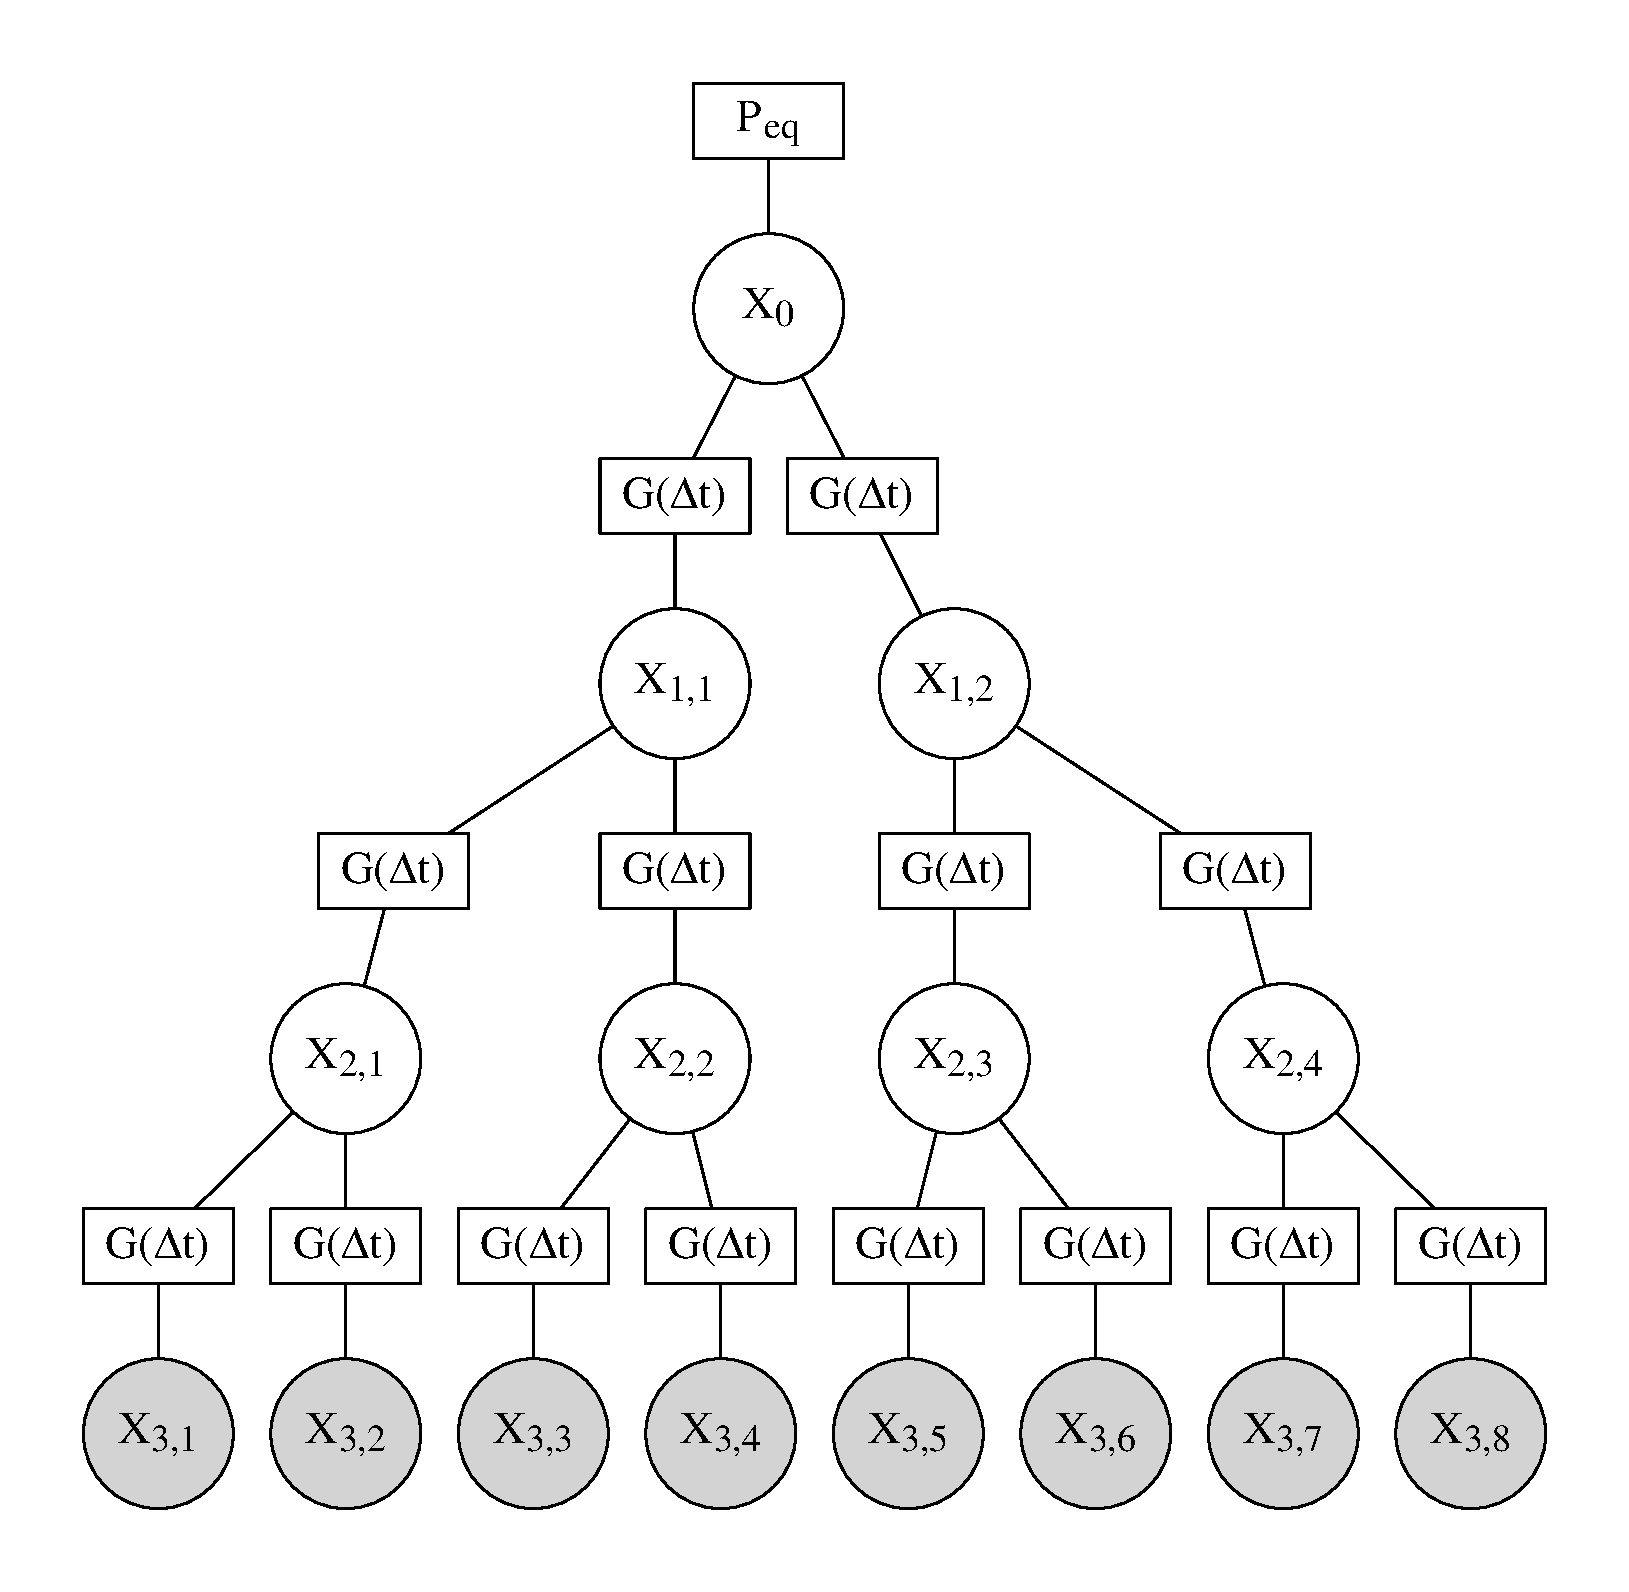
\includegraphics[width=0.65\textwidth]{Images/factgraph.pdf}
\end{center}
\caption{ Phylogenetic model for genetic drifting \label{fig:factgraph}}
\end{figure*}

Following standard Belief Propagation method \cite{}, the exact free energy (likelihood) of the model can be written in terms of two variables joint distributions $b(x_1,x_2)$, when $x_1$ and $x_2$ are first neighbors in the graph, and one variable distributions $b(x)$, as 
\begin{eqnarray*} 
F[\{b(\cdot) \}] &=& \sum_{(i-j)}  \sum_{x_i,x_j} \displaystyle\left( E_{i,j}(x_i,x_j) b_{i,j}(x_i,x_j) + b_{i,j}(x_i,x_j) \log b_{i,j}(x_i,x_j) \right)  \\
&& -2 \sum_{i}   \sum_{x_i,x_j} \left( E_{i}(x_i) b_{i}(x_i) + b_{i}(x_i) \log b_{i}(x_i) \right)
\end{eqnarray*}

The consistency between both types of distributions, when they share the same variable implies 
\[ b(x_1) = \sum_{x_2} b(x_1, x_2)
\]
and is guaranteed by a set of lagrange multipliers $m_{2 \to 1}(x_1)$ for every posible marginalization constraint.

\begin{figure*}[!htb]
\begin{center}
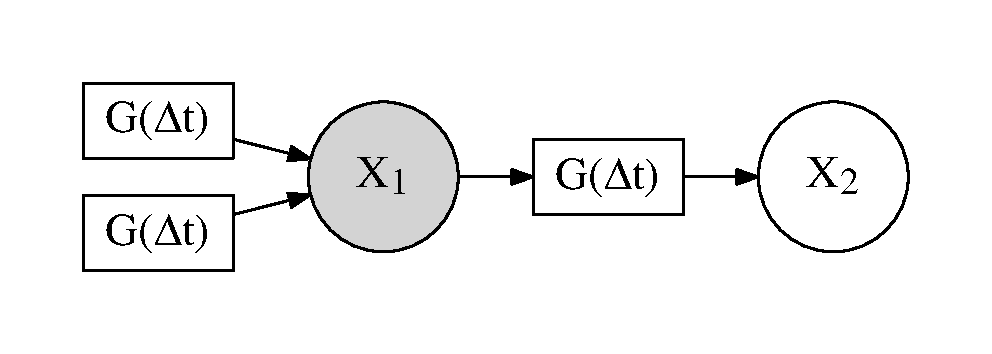
\includegraphics[width=0.65\textwidth]{Images/mess.pdf}
\end{center}
\caption{Message passing step \label{fig:mess}}
\end{figure*}

After introducing the messages in the free energy, we get a Lagrangian, and extremization in terms of beliefs give the relation
\begin{eqnarray}
b_{x_1,x_2} &=& \frac 1 {Z_{1,2}} G_{\Delta t}(x_1,x_2) \prod_{j\in \partial 1\setminus 2} m_{j\to 1}(x_1)  \:\prod_{j\in \partial 2\setminus 1} m_{j\to 2}(x_2) \\
b_{x_1} &=&  \frac 1 {Z_{1}}  \prod_{j\in \partial 1} m_{j\to 1}(x_1)  
\end{eqnarray}
Replacing this relations in the free energy, we get a ``variational'' free energy in terms of the messages that appear in the normalization constants:
\[ F[\{m_{a\to b} \}] = \sum_{(i-j)} Z_{i,j}[\{m\}] - 2 \sum_{i} Z_i[\{m\}] \]
Variational here means that the true values of $m_{i\to j}$ are the one solving 
\[\frac{\partial F[\{m\}]}{\partial m} = 0\]
resulting in 
\[ m_{1\to 2}(x_2) = \int \ud x_1 G_{\Delta t}(x_1,x_2) m_{i,\to 1}(x_1) m_{j,\to 1}(x_1)  \]
Assuming that messages are gaussians (not necessarily normalized)
\[ m(x) = \exp\left( -\frac 1 2 \vec x^T A \vec x + \vec B\cdot x\right)\]
and the propagator
\[G_{\Delta t} (x_1,x_2) = \exp\left( -\frac 1 2 [ x_1^T \Sigma^{-1} x_1 + x_2^T \Sigma^{-1} x_2 - 2 x_1^T (\Lambda \Sigma^{-1}) x_2 ] 
\right)\]
then the message passing step is only the following update
\begin{eqnarray*}
 m_{1\to 2}(x_2) &=& \int \ud x_1  \exp\left( -\frac 1 2 [ x_1^T \Sigma^{-1} x_1 + x_2^T \Sigma^{-1} x_2 - 2 x_1^T (\Lambda \Sigma^{-1}) x_2 ] 
-\frac 1 2 x_1^T A x_1 + \vec B^T x_1\right)  \\
&=& \exp\left( -\frac 1 2  x_2^T \Sigma^{-1} x_2 \right) \int \ud x_1  \exp\left( -\frac 1 2 x_1^T (\Sigma^{-1} + A) x_1 + x_1^T (B + (\Lambda \Sigma^{-1}) x_2) \right)  \\
&=&\exp\left( -\frac 1 2  x_2^T \Sigma^{-1} x_2 \right)  \exp\ -\frac 1 2 \left(  (B + (\Lambda \Sigma^{-1})x_2)^T (\Sigma^{-1} + A)^{-1}  (B + (\Lambda \Sigma^{-1}) x_2) \right) \\
&=&\exp\left( -\frac 1 2  x_2^T \left[ \Sigma^{-1} +(\Lambda \Sigma^{-1})^T (\Sigma^{-1} + A)^{-1}(\Lambda \Sigma^{-1}) \right] x_2   -B^T  (\Sigma^{-1} + A)^{-1}   (\Lambda \Sigma^{-1}) x_2 \right) 
\end{eqnarray*}
Calling $A = A_{i\to 1} + A_{j\to 1}$ y  $B = B_{i\to 1} + B_{j\to 1}$, the message update rule is
\begin{eqnarray*}
 A_{1\to 2} =  \Sigma^{-1} +(\Lambda \Sigma^{-1})^T (\Sigma^{-1} + A)^{-1}(\Lambda \Sigma^{-1})  \\
 B_{1 \to 2} = B^T  (\Sigma^{-1} + A)^{-1}   (\Lambda \Sigma^{-1}) 
\end{eqnarray*}
Such update step has to be implemented $3*N$, where $N$ is the number of free variables in the tree (not considering the observed leaves). Since the graph is a tree, there is no need for a fixed point iteration. If the procedure is carried from the leaves inwards, it will solve all messages in a single swept.


\subsection{Inverse problem: learning $C$}

Based on the exactness of the Bethe Free Energy for a tree, then 
\[ F[\{m\}] = - \log Z
\]
where 
\[ Z[x^k] = \int_{x_0,x_1,x_2,\ldots} \Psi(x_0) G(x_0,x_1) G(x_0,x_2) G(x_1,x_3) G(x_1,x_4) \ldots G...
\]
is the partition function but also the likelihood of the data at level $k$. For this reason, $F[\{m\}]$ is the log-likelihood, and a model can be
learned by maximizing it with respect to parameters. 

\section{Maximum likelihood} % (fold)
\label{sec:maximum_likelihood}

\subsection{Expression of the likelihood} % (fold)
\label{sub:expression_of_the_likelihood}

The full system, \ie all nodes in the tree, will be noted $\vec{X} = \{X_i\}_{i=1\ldots N}$. Each $X_i$ is a gaussian vector. $X_0$ is the root of the tree. We decompose the nodes in two groups, leaves and internal nodes: $\vec{X} = \{\vec{X}_h,\vec{X}_d\}$, with $\vec{X}_h$ being the internal nodes and $\vec{X}_d$ being the leaves. \\
The assumption on the distribution of $\vec{X}$ is that it follows the Ornstein-Uhlenbeck process, that is 
\begin{equation}
  \label{eq:ML_OU}
  \begin{split}
    P^0(X_i) &\propto \exp-\frac{1}{2}\left\{ X_i\bm{C}^{-1}X_i \right\}\\
    P^0(X_j|X_i;\Delta t) &\propto \exp-\frac{1}{2}\left\{ X_j\Sig^{-1}X_j + X_i\Lam^2\Sig^{-1} X_i - 2 X_i \Lam\Sig^{-1} X_j \right\}
  \end{split}
\end{equation}
The probability of a configuration $\vec{X}$ of the full system can be written as 
$$ P^0(\vec{X}) = P^0(X_0)P^0(X_1|X_0)P^0(X_2|X_0)P^0(X_3|X_1)P^0(X_4|X_1)\ldots $$
assuming the above mentionned pairwise tree topology. Expanding this expression, it is easy to see that probability $P^0$ can be written as
\begin{equation}
  \label{eq:ML_PairwiseDistribution}
  P^0(\vec{X}) = \frac{1}{Z^0}\exp\left\{ \sum_{i<j}X_iJ_{ij}X_j + \sum_{i=1}^N X_iH_iX_i  \right\}
\end{equation}
where 
\begin{equation*}
J_{ij} =
\begin{cases}
\Lam\Sig^{-1} & \text{if $i$ and $j$ are in contact} ,\\
0 & \text{otherwise}.
\end{cases}
\end{equation*}
and 
\begin{equation*}
H_i = -\frac{1}{2}\cdot
\begin{cases}
(1+\Lam^2)\Sig^{-1} & \text{if $i=0$},\\
\Sig^{-1} & \text{if $i$ is a leaf},\\
(1+2\Lam^2)\Sig^{-1} & \text{otherwise}.
\end{cases}
\end{equation*}
In other words, the system is described by a pairwise hamiltonian 
\begin{equation}
   \label{eq:ML_H0}
   \mathcal{H}^0 = -\sum_{i<j}X_iJ_{ij}X_j - \sum_{i=1}^N X_iH_iX_i.   
\end{equation}

It is important to note that thanks to the properties of the OU process, one can write the single and pairwise marginals of $P^0$. Indeed, using \ref{eq:ML_OU} immediatly gives
\begin{equation}
  \label{eq:ML_Fullmarginals}
  \begin{split}
    P^0_i(X_i) &\propto \exp-\frac{1}{2}\left\{ X_i\bm{C}^{-1}X_i \right\}\\
    P^0_{ij}(X_i,X_j;\Delta t) &\propto \exp-\frac{1}{2}\left\{ X_i\Sig^{-1} X_i + X_j\Sig^{-1}X_j - 2 X_i \Lam\Sig^{-1} X_j \right\}
  \end{split}
\end{equation}
This, put together with the fact that the topology of interaction of $J_{ij}$ is a tree, means we can write the free energy exactly using Bethe's formula
\begin{equation}
  \label{eq:ML_F0}
  \begin{split}
  -\log Z^0  =&\langle H^0\rangle_{P^0} - S(P^0)\\
   =& \sum_{i<j}\int_{X_i,X_j} P^0_{ij}(X_i,X_j)\left[\log P^0_{ij}(X_i,X_j) - X_iJ_{ij}X_j\right]\\
   & + \sum_{i=1}^N\int_{X_i} P^0_i(X_i)\left[-(r_i-1)\log P^0_i(X_i) - X_iH_iX_i\right]\\
   =& \sum_{i<j}\int_{X_i,X_j} P^0_{ij}(X_i,X_j)\left[\log P^0_{ij}(X_i,X_j) + E_{ij}(X_i,X_j)\right]\\
   & - \sum_{i=1}^N(r_i-1)\int_{X_i} P^0_i(X_i)\left[\log P^0_i(X_i) + E_i(X_i)\right],
  \end{split}
\end{equation}
by defining $E_{ij}(X_i,X_j) = - X_iJ_{ij}X_j + X_iH_iX_i + X_jH_jX_j$ and $E_i(X_i) = -X_iH_iX_i$.

Let us now write the probability of observing a certain configuration $\vec{X_d}$ of the leaves. The likelihood is 
\begin{equation}
  \label{eq:ML_likelihood}
  \begin{split}
  P(\vec{X}_d | \bm{C}) =& \log \int_{\vec{X}_h} P^0(\vec{X})\\
               =& -\log Z^0 + \log\int_{\vec{X}_h} e^{-\mathcal{H}^0(\vec{X}_h,\vec{X}_d)}.
  \end{split}
\end{equation}
The first member of the right hand side is the free energy associated to $\mathcal{H}^0$, described by equation \ref{eq:ML_F0}. The second member is the sum of Boltzmann weights over a sub ensemble of the system, with leaves fixed to a given configuration. This can be seen as the partition function of a second hamiltonian $\mathcal{H}^d(\vec{X}_h) = \mathcal{H}^0(\vec{X}_h,\vec{X}_d)$. Analytical expression of $\mathcal{H}^d$ can easily be written
\begin{equation}
  \label{eq:ML_Hd}
  \mathcal{H}^d(\vec{X}_h) = -\sum_{1\leq i<j\leq N_h}X_iJ_{ij}X_j - \sum_{i=1}^{N_h} \left(X_iH_iX_i + \mu_i X_i\right),
\end{equation}
where the fields and couplings $\{J_{ij},H_i\}$ are equal to those of $\mathcal{H}^0$, and 
\begin{equation*}
  \label{eq:ML_mudef}
  \mu_i =
  \begin{cases}
  (X_i^{(1)} + X_i^{(2)})\Lam\Sig^{-1} & \text{if $i$ is in contact with two leaves $X_i^{(1)}$ and $X_i^{(2)}$} ,\\
  0 & \text{otherwise}.
  \end{cases}
\end{equation*}
As a consequence, the likelihood can be written as 
\begin{equation}
  \label{eq:ML_likelihood2}
  P(\vec{X}_d | \bm{C}) = \log Z^d -\log Z^0.
\end{equation}
The second member of this equation can be computed using the analytical formula \ref{eq:ML_F0}. Since the hamiltonian $\mathcal{H}^d$ is also pairwise, and with a tree-like topology of interaction, we can also write its free energy using the Bethe approximation. However, in this case, we do not know the pairwise marginals $P_{ij}^d(X_i,X_j)$. Thus, we will use message passing to compute those and write the free energy. \\

% subsection expression_of_the_likelihood (end)

\subsection{Gradient of $Z^0$} % (fold)
\label{sub:gradient_of_z_0_}
The free energy of $\mathcal{H}^0$ can be expressed as a sum of pairwise free energies $F_{ij}^0$ and single site free energies $F_i^0$. Expanding equation \ref{eq:ML_F0} using definitions of couplings $J_{ij}$ and fields $H_i$ as well as the characteristics of the Ornstein-Uhlenbeck process, one finds 
\begin{equation}
  F^0 = -\sum_{i<j}\log{Z_{ij}^0} + \sum_{i=1}^N\log Z_i^0,
\end{equation}
where 
\begin{equation}
  \label{eq:ML_localZ0}
  \begin{split}
    Z_{i}^0 =& \int\ddroit X_i \exp-\frac{1}{2}X_i\bm{C}^{-1}X_i\\
    Z_{ij}^0 =& \int\ddroit X_i \ddroit X_j \exp-\frac{1}{2}\left\{ X_i\Sig^{-1}X_i + X_j\Sig^{-1}X_j - 2 X_i\Lam\Sig^{-1}X_j \right\}.
  \end{split}
\end{equation}


% subsection gradient_of_z_0_ (end)

\subsection{Message passing} % (fold)
\label{sub:message_passing}

Message from $i$ to $j$, in the case that $i$ is a leaf of the tree
\begin{equation}
  \begin{split}
    m_{ij}(X_j) =& \int\ddroit X_i e^{X_iH_iX_i + (X_jJ_{ij} + \mu_i)X_i}\prod_{k\in\partial i\setminus j}m_{ki}(X_i)\\
                =& \left( \frac{\pi^L}{\vert H_i\vert} \right)^{1/2}e^{-\frac{1}{4}(X_jJ_{ij} + \mu_i)H_i^{-1}(J_{ij}X_j+\mu_i)}.
  \end{split}
\end{equation}
From this, it is clear that messages will always be a gaussian function of their variable, since integrating products of gaussian functions always yields a new gaussian function. Thus, we can write messages in the following way
\begin{equation}
  m_{ij}(X_j) \propto e^{X_j\Phi_{ij}X_j + \Psi_{ij}X_j}
\end{equation}
Plugging this into the message defining equation, we obtain
\begin{equation}
  \begin{split}
  m_{ij}(X_j) =& \int\ddroit X_i e^{X_iH_iX_i + (X_jJ_{ij} + \mu_i)X_i}\prod_{k\in\partial i\setminus j}m_{ki}(X_i)\\
              \propto& \int\ddroit X_i \exp\left\{\left(X_jJ_{ij}+\mu_i + \sum_{k\in\partial i\setminus j}\Psi_{ki}\right)X_i + X_i\left(H_i + \sum_{k\in\partial i\setminus j}\Phi_{ki}\right)X_i \right\}
  \end{split}
\end{equation}
and thus arriving to the following recurrence relation after performing the integration
\begin{equation}
\begin{split}
  \Phi_{ij} =& -\frac{1}{4} J_{ij}\left( H_i + \sum_{k\in\partial i\setminus j}\Phi_{ki} \right)^{-1}J_{ij}\\
  \Psi_{ij} =& -\frac{1}{2}J_{ij}\left(H_i + \sum_{k\in\partial i\setminus j}\Phi_{ki}\right)^{-1}\left(\mu_i+\sum_{k\in\partial i\setminus j}\Psi_{ki}\right)
\end{split}
\end{equation}
% subsection message_passing (end)

% section maximum_likelihood (end)

\section{Annex} % (fold)
\label{sec:annex}
\subsection{Gaussian integration} % (fold)
\label{sub:gaussian_integration}
\begin{equation*}
  Z_{12} =\int\ddroit X_1 \ddroit X_2 \exp\left\{ X_1A_{11}X_1 + X_2A_{22}X_2 + X_1A_{12}X_2 + B_1X_1 + B_2X_2 \right\}
\end{equation*}
can be written as 
\begin{equation}
\begin{split}
  Z_{12}=&\int\ddroit \bm{Y} \exp-\frac{1}{2}(\bm{Y}-\bm{m})\bm{K}(\bm{Y}-\bm{m})\cdot\exp\left(2\bm{m}\bm{K}\bm{m}\right)\\
  =& \left(\frac{(2\pi)^{2L}}{\vert \bm{K}\vert}\right)\cdot\exp\left(2\bm{m}\bm{K}\bm{m}\right)
\end{split}
\end{equation}  
where 
\begin{equation*}
  \bm{Y} = \left(
  \begin{array}{c}
    X_1\\
    X_2
  \end{array}
  \right)\quad
  \bm{K} = -\left(
  \begin{array}{cc}
    2A_{11}& A_{12}\\
    A_{12}& 2A_{22}
  \end{array}
  \right)\quad\text{and}\quad
  \bm{m}=\left(
  \begin{array}{c}
    B_2A_{12} - 2B_1A_{22}\\
    B_1A_{12} - 2B_2A_{11}
  \end{array}
  \right).*(4A_{22}A_{11}-A_{12}^2)^{-1}
\end{equation*}
% \begin{equation*}
%   \begin{split}
%     Z_{12} =&\int\ddroit X_1 \ddroit X_2 \exp\left\{ X_1A_{11}X_1 + X_2A_{22}X_2 + X_1A_{12}X_2 + B_1X_1 + B_2X_2 \right\}\\
%     % =& \left(\right)
  
%   \end{split}
% \end{equation*}

% subsection gaussian_integration (end)
% section annex (end)


\bibliography{bib_phylo}
\bibliographystyle{unsrt}



\end{document}

\end{document}
=============

